\documentclass{standalone}
\usepackage{tikz}
\usetikzlibrary{patterns, positioning}


\begin{document}
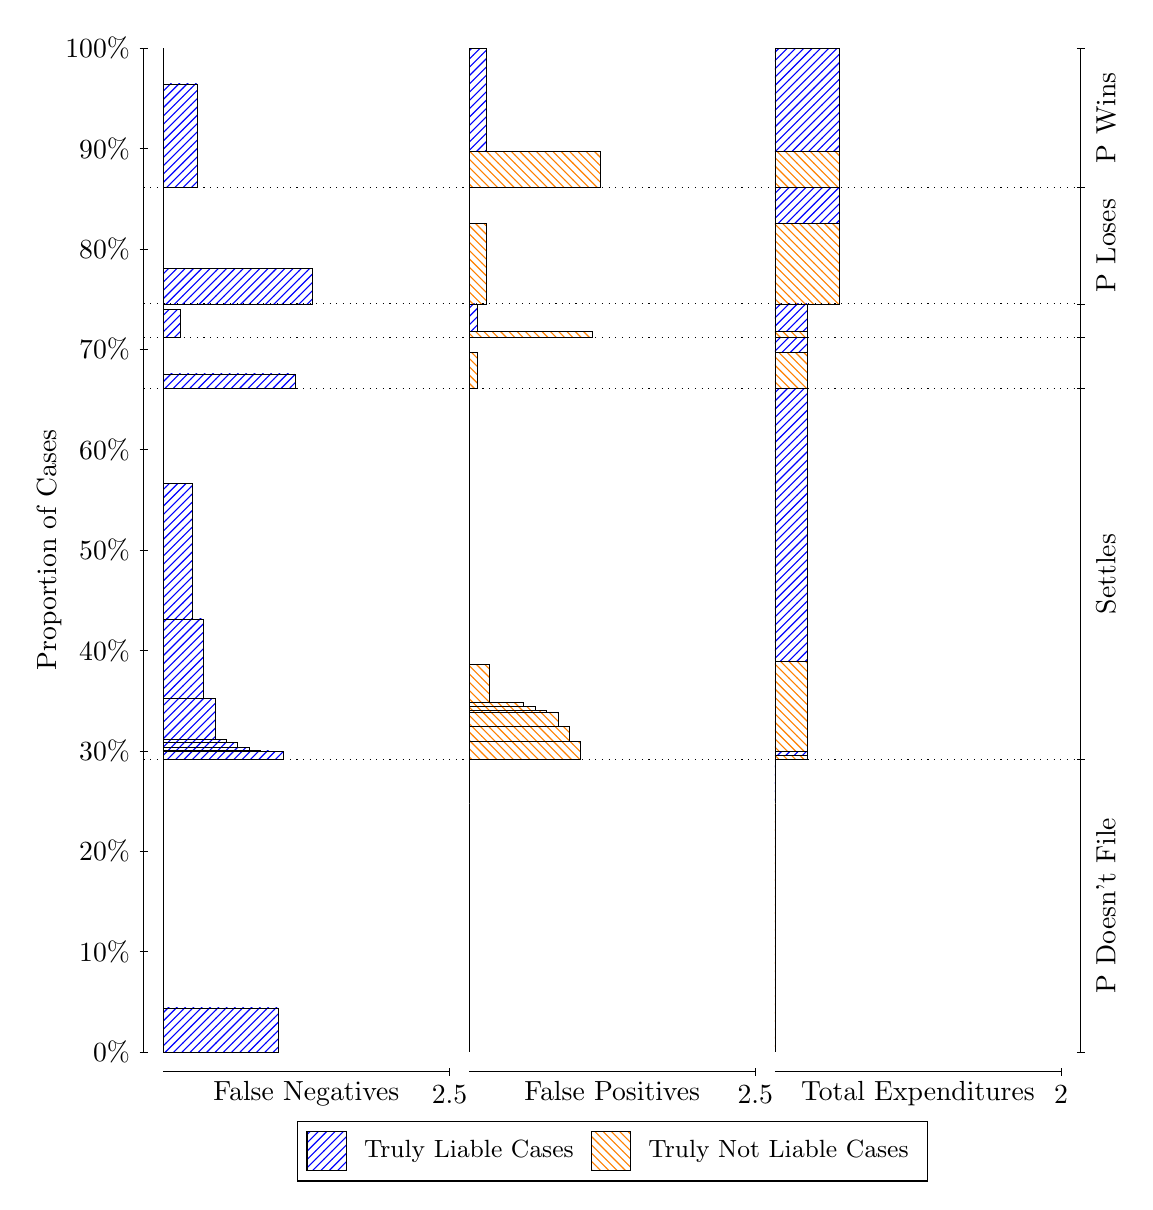
\begin{tikzpicture}
\draw[black, very thin] (1.5,1.75) -- (1.5,14.5);
\node[rotate=90, text=black, anchor=center] at (0.3, 8.125) {Proportion of Cases};
\draw[black, very thin] (1.45,1.75) -- (1.55,1.75);
\node[text=black, anchor=east] at (1.45, 1.75) {0\%};
\draw[black, very thin] (1.45,3.025) -- (1.55,3.025);
\node[text=black, anchor=east] at (1.45, 3.025) {10\%};
\draw[black, very thin] (1.45,4.3) -- (1.55,4.3);
\node[text=black, anchor=east] at (1.45, 4.3) {20\%};
\draw[black, very thin] (1.45,5.575) -- (1.55,5.575);
\node[text=black, anchor=east] at (1.45, 5.575) {30\%};
\draw[black, very thin] (1.45,6.85) -- (1.55,6.85);
\node[text=black, anchor=east] at (1.45, 6.85) {40\%};
\draw[black, very thin] (1.45,8.125) -- (1.55,8.125);
\node[text=black, anchor=east] at (1.45, 8.125) {50\%};
\draw[black, very thin] (1.45,9.4) -- (1.55,9.4);
\node[text=black, anchor=east] at (1.45, 9.4) {60\%};
\draw[black, very thin] (1.45,10.675) -- (1.55,10.675);
\node[text=black, anchor=east] at (1.45, 10.675) {70\%};
\draw[black, very thin] (1.45,11.95) -- (1.55,11.95);
\node[text=black, anchor=east] at (1.45, 11.95) {80\%};
\draw[black, very thin] (1.45,13.225) -- (1.55,13.225);
\node[text=black, anchor=east] at (1.45, 13.225) {90\%};
\draw[black, very thin] (1.45,14.5) -- (1.55,14.5);
\node[text=black, anchor=east] at (1.45, 14.5) {100\%};

\draw[black, very thin] (13.4,1.75) -- (13.4,14.5);
\draw[black, very thin] (13.35,1.75) -- (13.45,1.75);
\node[anchor=west] at (13.35, 1.75) {};
\draw[black, very thin] (13.35,5.4625) -- (13.45,5.4625);
\node[anchor=west] at (13.35, 5.4625) {};
\draw[black, very thin] (13.35,10.175) -- (13.45,10.175);
\node[anchor=west] at (13.35, 10.175) {};
\draw[black, very thin] (13.35,10.822) -- (13.45,10.822);
\node[anchor=west] at (13.35, 10.822) {};
\draw[black, very thin] (13.35,11.252) -- (13.45,11.252);
\node[anchor=west] at (13.35, 11.252) {};
\draw[black, very thin] (13.35,12.729) -- (13.45,12.729);
\node[anchor=west] at (13.35, 12.729) {};
\draw[black, very thin] (13.35,14.5) -- (13.45,14.5);
\node[anchor=west] at (13.35, 14.5) {};

\draw[black, very thin, pattern color=blue, pattern=north east lines] (1.75,1.75) rectangle (3.2033,2.3088);
\draw[black, very thin, pattern color=orange, pattern=north west lines] (1.75,2.3088) rectangle (1.75,5.4625);
\draw[black, very thin, pattern color=blue, pattern=north east lines] (1.75,5.4625) rectangle (3.276,5.57);
\draw[black, very thin, pattern color=blue, pattern=north east lines] (1.75,5.57) rectangle (3.1307,5.5736);
\draw[black, very thin, pattern color=blue, pattern=north east lines] (1.75,5.5736) rectangle (2.9853,5.5772);
\draw[black, very thin, pattern color=blue, pattern=north east lines] (1.75,5.5772) rectangle (2.84,5.6146);
\draw[black, very thin, pattern color=blue, pattern=north east lines] (1.75,5.6146) rectangle (2.6947,5.6808);
\draw[black, very thin, pattern color=blue, pattern=north east lines] (1.75,5.6808) rectangle (2.5493,5.7214);
\draw[black, very thin, pattern color=blue, pattern=north east lines] (1.75,5.7214) rectangle (2.404,6.2423);
\draw[black, very thin, pattern color=blue, pattern=north east lines] (1.75,6.2423) rectangle (2.2587,7.2489);
\draw[black, very thin, pattern color=blue, pattern=north east lines] (1.75,7.2489) rectangle (2.1133,8.9671);
\draw[black, very thin, pattern color=orange, pattern=north west lines] (1.75,8.9671) rectangle (1.75,10.175);
\draw[black, very thin, pattern color=blue, pattern=north east lines] (1.75,10.175) rectangle (3.4213,10.362);
\draw[black, very thin, pattern color=orange, pattern=north west lines] (1.75,10.362) rectangle (1.75,10.822);
\draw[black, very thin, pattern color=blue, pattern=north east lines] (1.75,10.822) rectangle (1.968,11.177);
\draw[black, very thin, pattern color=orange, pattern=north west lines] (1.75,11.177) rectangle (1.75,11.252);
\draw[black, very thin, pattern color=blue, pattern=north east lines] (1.75,11.252) rectangle (3.6393,11.706);
\draw[black, very thin, pattern color=orange, pattern=north west lines] (1.75,11.706) rectangle (1.75,12.729);
\draw[black, very thin, pattern color=blue, pattern=north east lines] (1.75,12.729) rectangle (2.186,14.044);
\draw[black, very thin, pattern color=orange, pattern=north west lines] (1.75,14.044) rectangle (1.75,14.5);
\draw[black, very thin, pattern color=orange, pattern=north west lines] (5.6333,1.75) rectangle (5.6333,4.9036);
\draw[black, very thin, pattern color=blue, pattern=north east lines] (5.6333,4.9036) rectangle (5.6333,5.4625);
\draw[black, very thin, pattern color=orange, pattern=north west lines] (5.6333,5.4625) rectangle (7.0503,5.696);
\draw[black, very thin, pattern color=orange, pattern=north west lines] (5.6333,5.696) rectangle (6.905,5.8814);
\draw[black, very thin, pattern color=orange, pattern=north west lines] (5.6333,5.8814) rectangle (6.7597,6.06);
\draw[black, very thin, pattern color=orange, pattern=north west lines] (5.6333,6.06) rectangle (6.6143,6.0886);
\draw[black, very thin, pattern color=orange, pattern=north west lines] (5.6333,6.0886) rectangle (6.469,6.1375);
\draw[black, very thin, pattern color=orange, pattern=north west lines] (5.6333,6.1375) rectangle (6.3237,6.1381);
\draw[black, very thin, pattern color=orange, pattern=north west lines] (5.6333,6.1381) rectangle (6.3237,6.1862);
\draw[black, very thin, pattern color=orange, pattern=north west lines] (5.6333,6.1862) rectangle (6.1783,6.1896);
\draw[black, very thin, pattern color=orange, pattern=north west lines] (5.6333,6.1896) rectangle (6.033,6.1943);
\draw[black, very thin, pattern color=orange, pattern=north west lines] (5.6333,6.1943) rectangle (5.8877,6.6703);
\draw[black, very thin, pattern color=blue, pattern=north east lines] (5.6333,6.6703) rectangle (5.6333,10.175);
\draw[black, very thin, pattern color=orange, pattern=north west lines] (5.6333,10.175) rectangle (5.7423,10.635);
\draw[black, very thin, pattern color=blue, pattern=north east lines] (5.6333,10.635) rectangle (5.6333,10.822);
\draw[black, very thin, pattern color=orange, pattern=north west lines] (5.6333,10.822) rectangle (7.1957,10.897);
\draw[black, very thin, pattern color=blue, pattern=north east lines] (5.6333,10.897) rectangle (5.7423,11.252);
\draw[black, very thin, pattern color=orange, pattern=north west lines] (5.6333,11.252) rectangle (5.8513,12.275);
\draw[black, very thin, pattern color=blue, pattern=north east lines] (5.6333,12.275) rectangle (5.6333,12.729);
\draw[black, very thin, pattern color=orange, pattern=north west lines] (5.6333,12.729) rectangle (7.3047,13.184);
\draw[black, very thin, pattern color=blue, pattern=north east lines] (5.6333,13.184) rectangle (5.8513,14.5);
\draw[black, very thin, pattern color=orange, pattern=north west lines] (9.5167,1.75) rectangle (9.5167,4.9036);
\draw[black, very thin, pattern color=blue, pattern=north east lines] (9.5167,4.9036) rectangle (9.5167,5.4625);
\draw[black, very thin, pattern color=orange, pattern=north west lines] (9.5167,5.4625) rectangle (9.9254,5.4631);
\draw[black, very thin, pattern color=blue, pattern=north east lines] (9.5167,5.4631) rectangle (9.9254,5.464);
\draw[black, very thin, pattern color=orange, pattern=north west lines] (9.5167,5.464) rectangle (9.9254,5.5202);
\draw[black, very thin, pattern color=blue, pattern=north east lines] (9.5167,5.5202) rectangle (9.9254,5.5638);
\draw[black, very thin, pattern color=orange, pattern=north west lines] (9.5167,5.5638) rectangle (9.9254,6.7148);
\draw[black, very thin, pattern color=blue, pattern=north east lines] (9.5167,6.7148) rectangle (9.9254,10.175);
\draw[black, very thin, pattern color=orange, pattern=north west lines] (9.5167,10.175) rectangle (9.9254,10.635);
\draw[black, very thin, pattern color=blue, pattern=north east lines] (9.5167,10.635) rectangle (9.9254,10.822);
\draw[black, very thin, pattern color=orange, pattern=north west lines] (9.5167,10.822) rectangle (9.9254,10.897);
\draw[black, very thin, pattern color=blue, pattern=north east lines] (9.5167,10.897) rectangle (9.9254,11.252);
\draw[black, very thin, pattern color=orange, pattern=north west lines] (9.5167,11.252) rectangle (10.334,12.275);
\draw[black, very thin, pattern color=blue, pattern=north east lines] (9.5167,12.275) rectangle (10.334,12.729);
\draw[black, very thin, pattern color=orange, pattern=north west lines] (9.5167,12.729) rectangle (10.334,13.184);
\draw[black, very thin, pattern color=blue, pattern=north east lines] (9.5167,13.184) rectangle (10.334,14.5);
\draw[black, dotted] (1.5,5.4625) -- (13.4,5.4625);
\draw[black, dotted] (1.5,10.175) -- (13.4,10.175);
\draw[black, dotted] (1.5,10.822) -- (13.4,10.822);
\draw[black, dotted] (1.5,11.252) -- (13.4,11.252);
\draw[black, dotted] (1.5,12.729) -- (13.4,12.729);
\draw[black, very thin] (1.75,1.5) -- (5.3833,1.5);
\node[text=black, anchor=north] at (3.5667, 1.5) {False Negatives};
\draw[black, very thin] (5.3833,1.45) -- (5.3833,1.55);
\node[text=black, anchor=north] at (5.3833, 1.45) {2.5};

\draw[black, very thin] (5.6333,1.5) -- (9.2667,1.5);
\node[text=black, anchor=north] at (7.45, 1.5) {False Positives};
\draw[black, very thin] (9.2667,1.45) -- (9.2667,1.55);
\node[text=black, anchor=north] at (9.2667, 1.45) {2.5};

\draw[black, very thin] (9.5167,1.5) -- (13.15,1.5);
\node[text=black, anchor=north] at (11.333, 1.5) {Total Expenditures};
\draw[black, very thin] (13.15,1.45) -- (13.15,1.55);
\node[text=black, anchor=north] at (13.15, 1.45) {2};

\node[text=black, centered, rotate=90] at (13.72, 3.6062) {P Doesn't File};
\node[text=black, centered, rotate=90] at (13.72, 7.8187) {Settles};


\node[text=black, centered, rotate=90] at (13.72, 11.99) {P Loses};
\node[text=black, centered, rotate=90] at (13.72, 13.614) {P Wins};

\draw (7.449999999999999,1.5) node[draw=none] (baseCoordinate) {};
\begin{scope}[align=center]
        \matrix[scale=0.5, draw=black, below=0.5cm of baseCoordinate, nodes={draw}, column sep=0.1cm]{
            \node[rectangle, draw, minimum width=0.5cm, minimum height=0.5cm, pattern color=blue, pattern=north east lines] {}; &
            \node[draw=none, font=\small, text=black] (B) {Truly Liable Cases}; &
            \node[rectangle, draw, minimum width=0.5cm, minimum height=0.5cm, pattern color=orange, pattern=north west lines] {}; &
            \node[draw=none, font=\small, text=black] (B) {Truly Not Liable Cases}; \\
            };
\end{scope}

\end{tikzpicture}
\end{document}